
\documentclass[ms.tex]{subfiles} 
\begin{document} 

\section{Introduction} 
\begin{itemize} 
	\item Nitrogen (N) is an element that traces slow neutron capture 
	(s-process) nucleosynthesis. To first order it's produced only in core 
	collapse supernovae (CCSNe) and asymptotic giant branch (AGB) stars 
	\citep{Johnson2019}. 

	\item The observed [N/O]-[O/H] relation in the gas phase is more or less 
	the same between different environments. 
	We demonstrate this in Fig.~\ref{fig:no_oh_observed} where we compile 
	measurements from previous studies interested in various astrophysical 
	systems. 

	\item Qualitatively, the rise in N abundances with increasing [O/H] can be 
	attributed to the metallicity-dependent nature of N yields from AGB stars 
	(\citealp{Vincenzo2016}; see also discussion in~\S~X). 

	\item How well do chemical evolution models for the Milky Way with various 
	``off-the-shelf'' yield models perform at reproducing this trend? 

	\item Nitrogen has considerable yields through~\textit{secondary} channels: 
	the processing of already produced metals into nitrogen. 
	\begin{itemize} 
		\item First and foremost is the CNO cycle, in which carbon (C), N, and 
		oxygen (O) catalyze the fusion of four protons into helium-4. The 
		reactions of the CNO cycle: 
		\begin{equation} 
		\Ctwelve(p,\gamma)\Nthirteen(\beta^+,\nu_e)\Cthirteen 
		(p,\gamma)\Nfourteen(p,\gamma)\Ofifteen(\beta^+,\nu_e)
		\Nfifteen(p,\alpha)\Ctwelve 
		\end{equation} 
		Due to a small cross section for proton capture, the 
		$\Nfourteen(p,\gamma)\Ofifteen$ reaction is particularly slow. 
		As a result, to first order the effect of the CNO cycle is to process 
		all of the available C and O into~\Nfourteen. 
	\end{itemize} 
\end{itemize} 

\begin{figure*} 
\centering 
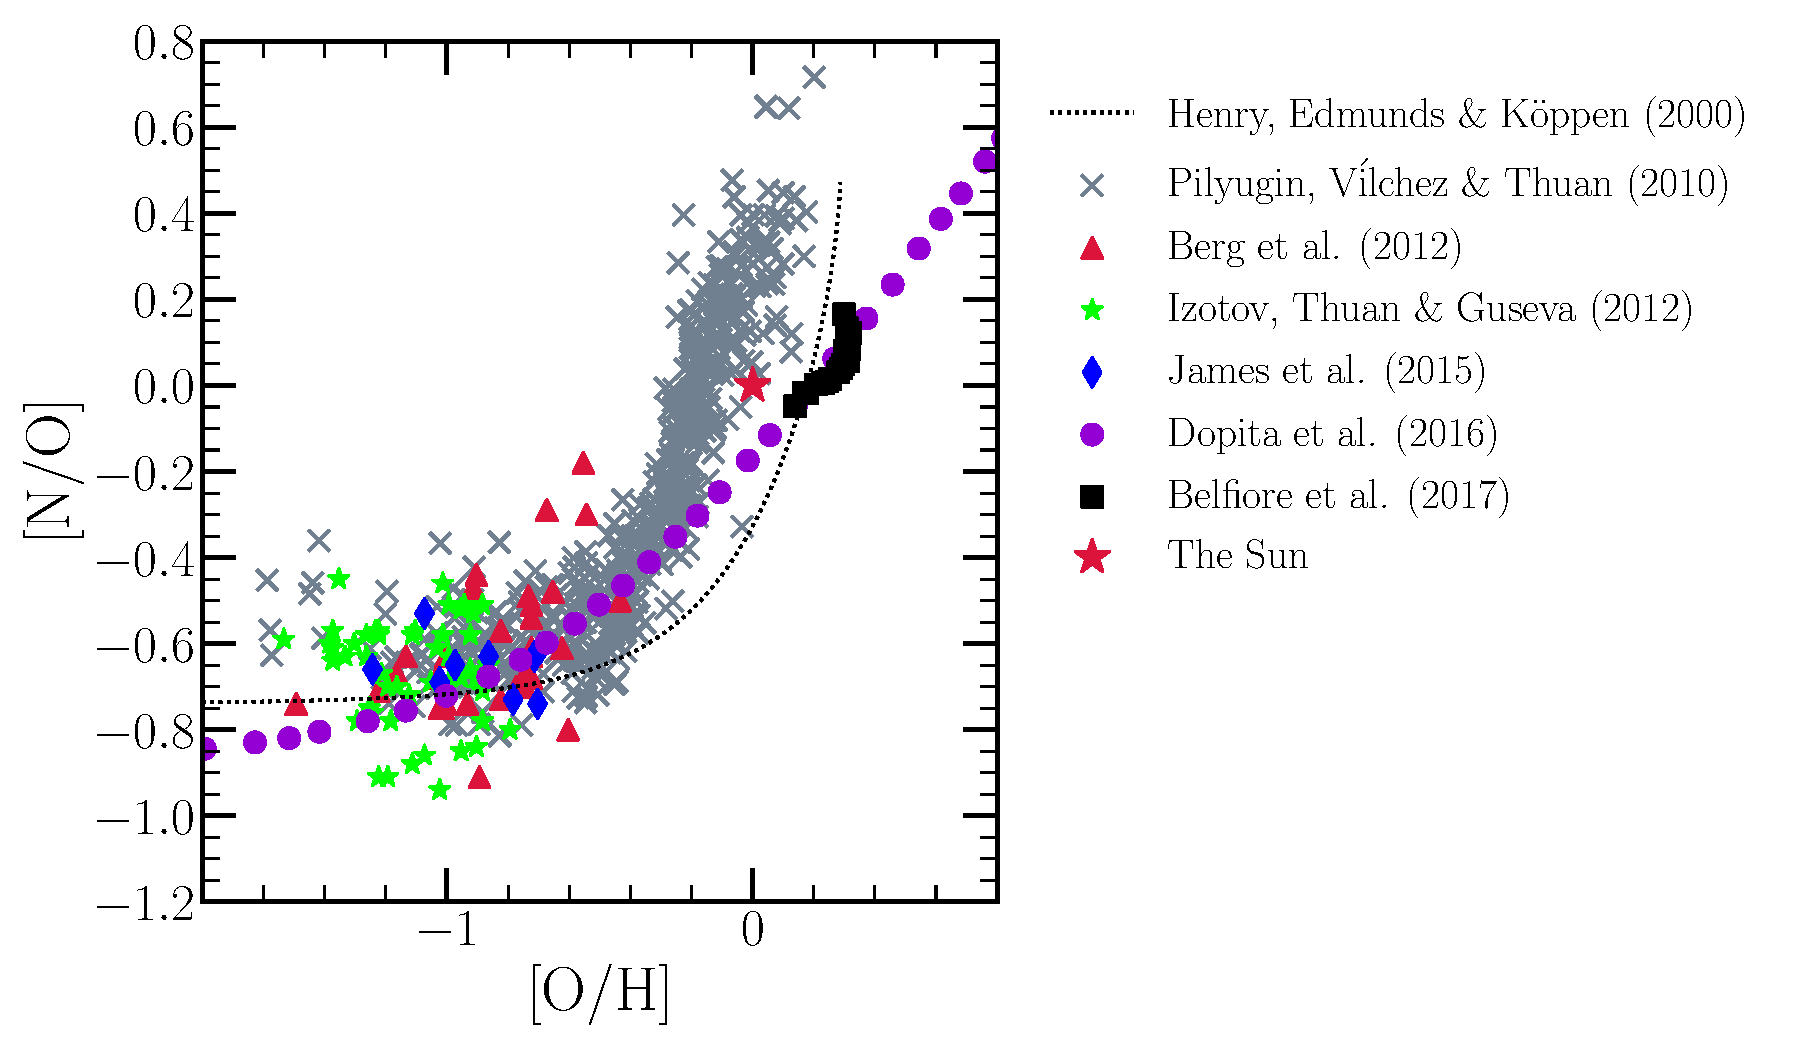
\includegraphics[scale = 0.5]{no_oh_observed.pdf} 
\caption{ 
The [N/O]-[O/H] relation observed in HII regions in nearby NGC spiral galaxies 
(grey X's:~\citealp*{Pilyugin2010}), in HII regions in blue, diffuse star 
forming dwarf galaxies (red triangles:~\citealp{Berg2012}; 
green stars:~\citealp*{Izotov2012}; blue diamonds:~\citealp{James2015}), in 
local stars and HII regions (purple circles:~\citealp{Dopita2016}), and in the 
MaNGA IFU survey (black squares:~\citealp{Belfiore2017}). 
The fit to [N/O] as a function of [O/H] in Galactic and extragalactic HII 
regions by~\citet*{Henry2000} is shown in a black dotted line. 
The Sun, at (0, 0) on this plot by definition, is marked by a red star. 
We omit the uncertainties for visual clarity. 
} 
\label{fig:no_oh_observed} 
\end{figure*} 

\begin{itemize} 
	\item Fig.~\ref{fig:no_oh_observed} presents a compilation of observed 
	abundances of N and O in the gas phase: 
	\begin{itemize} 
		\item HII regions in nearby NGC spirals~\citep{Pilyugin2010} 

		\item HII regions in blue, diffuse star forming dwarf 
		galaxies~\citep{Berg2012, Izotov2012, James2015} 

		\item Local stars and HII regions~\citep{Dopita2016} 

		\item Galactic and extragalactic HII regions~\citep{Henry2000} 

		\item Star-forming regions in 550 nearby galaxies in the MaNGA IFU 
		survey~\citep{Belfiore2017} 
	\end{itemize} 
	Despite intrinsic scatter and some systematic variation in how the 
	abundances are determined, the [N/O]-[O/H] relation is more or less the 
	same across a wide range of physical enrivonments. 

	\item In this paper, we're interested in the origin of both the shape and 
	scatter in this trend. 

	\item In a sample of 6,507 galaxies from the Mapping Galaxies at Apache 
	Point Observatory survey~\citep[MaNGA;][]{Bundy2015},~\citet{Schaefer2020} 
	recently argued that intrinsic scatter in the [N/O]-[O/H] relation 
	near and above solar metallicity is a consequence of variations in the 
	local star formation efficiency. In regions of slower star formation, the 
	[N/O] ratio tends to be slightly higher at fixed [O/H] (see their Fig. 4), 
	as expected from chemical evolution models~\citep[e.g.][]{Molla2006, 
	Vincenzo2016}. 
\end{itemize} 

\end{document} 

